\pgfplotstableread{data/tableinsert.dat}\mytableinsert
\pgfplotstableread{data/tablefind.dat}\mytablefind

\begin{figure*}[ht]
  \begin{adjustbox}{width=\textwidth}
    \centering
    \begin{subfigure}{\columnwidth}
      \centering
      \begin{tikzpicture}[scale=0.9]
        \begin{axis}[xlabel=N Threads, ylabel=Latency (usec), ymin=0, scaled ticks=false, tick label style={/pgf/number format/fixed},
            boxplot/draw direction=y,
            ytick distance={0.1},
            ymax={0.6},
            cycle list={{red},{blue},{black}},
            legend pos={north west}
          ]
          % hack to make legend
          \addlegendimage{area legend,fill=red,draw=black}; \addlegendentry{arr};
          \addlegendimage{area legend,fill=blue,draw=black}; \addlegendentry{ch};
          \addlegendimage{area legend,fill=black,draw=black}; \addlegendentry{tbb};

          \pgfplotsinvokeforeach{3,...,23}{
            \addplot+[boxplot prepared from table={table=\mytableinsert,
              row=#1, lower whisker=lw, upper whisker=uw, lower quartile=lq, upper quartile=uq,
            median=med, draw position=nthreads}, boxplot prepared] coordinates {};
          }
        \end{axis}
      \end{tikzpicture}
      \caption{Latency per successful \texttt{insert}.}
    \end{subfigure}

    \begin{subfigure}{\columnwidth}
      \centering
      \begin{tikzpicture}[scale=0.9]
        \begin{axis}[xlabel=N Threads, ylabel=Latency (usec), ymin=0, scaled ticks=false, tick label style={/pgf/number format/fixed},
            boxplot/draw direction=y,
            ytick distance={0.1},
            ymax={0.6},
            cycle list={{red},{blue},{black}},
            legend pos={north west}
          ]
          % hack to make legend
          \addlegendimage{area legend,fill=red,draw=black}; \addlegendentry{arr};
          \addlegendimage{area legend,fill=blue,draw=black}; \addlegendentry{ch};
          \addlegendimage{area legend,fill=black,draw=black}; \addlegendentry{tbb};

          \pgfplotsinvokeforeach{3,...,23}{
            \addplot+[boxplot prepared from table={table=\mytablefind,
              row=#1, lower whisker=lw, upper whisker=uw, lower quartile=lq, upper quartile=uq,
            median=med, draw position=nthreads}, boxplot prepared] coordinates {};
          }
        \end{axis}
      \end{tikzpicture}
      \caption{Latency per fail \texttt{insert} followed by an \texttt{erase}.}
    \end{subfigure}
  \end{adjustbox}

  \caption{Latency of our hash-table implementation (\textit{arr}) in comparison
  to libcuckoo (\textit{ch}) and tbb concurrent hash map (\textit{tbb}).  Each
  hash-table is initiailzied with the initial size of $2^{16}$, the number of
  insertion per thread is chosen so that there is enough room and no expansion is
  required. TBB is also compiled with \textit{tbb-malloc} to improve performance.
  Latency exceeds an 0.5 microsecond is not shown.\label{fig:hash-table}}

\end{figure*}

\subsection{Runtime Overhead}
In this section, we evaluate empirically each components of our runtime and
justify the overhead that we have previously estimated.

\subsubsection{Concurrent Hash-Table}
To evaluate the overhead due to hash-table operations, we measure the latency 
on hash-table operations in the two following scenarios when performing them
in a number of POSIX threads:

\begin{itemize}
  \item A thread performs \texttt{insert} when there is no item with the same key.
  \item A thread performs \texttt{insert} and there is already items in the hash-table, and it subsequently
    performs \texttt{erase}.
\end{itemize}

 The two scenarious represent the only two possible runtime execution of the
 hash-table in our algorithms, thus measuring the latency in both cases give us
 an idea on how it will add to the overhead of MPI procedure. To justify the
 benefit of customization, we also compare ourselves to two popular general
 purposes hash-tables: libcuckoo implementing cuckoo hashing (\textit{ch})
 \cite{chasing}, and TBB concurrent hashmap (\textit{tbb}) \cite{tbb}.

Figure~\ref{fig:hash-table} shows the result of our experiment. In both cases,
both TBB concurrent hash map and libcuckoo shows inconsistent latency when
there is more concurrent threads, which is the result of conflicts. Since our
hash-table is optimized for these patterns, our latency is almost always as low
as 50 nanosecond. This latency is consitent with our expectation that our cost
for the hash-table is equivalent to 2 memory writes.

\subsubsection{Concurrent Packet Pool}
We describe here an experiment to evaluate the overhead due to packet pool.

\subsubsection{Thread scheduler}
\subsubsection{Overall latency for single-threaded case}
\begin{figure}
  \centering 
  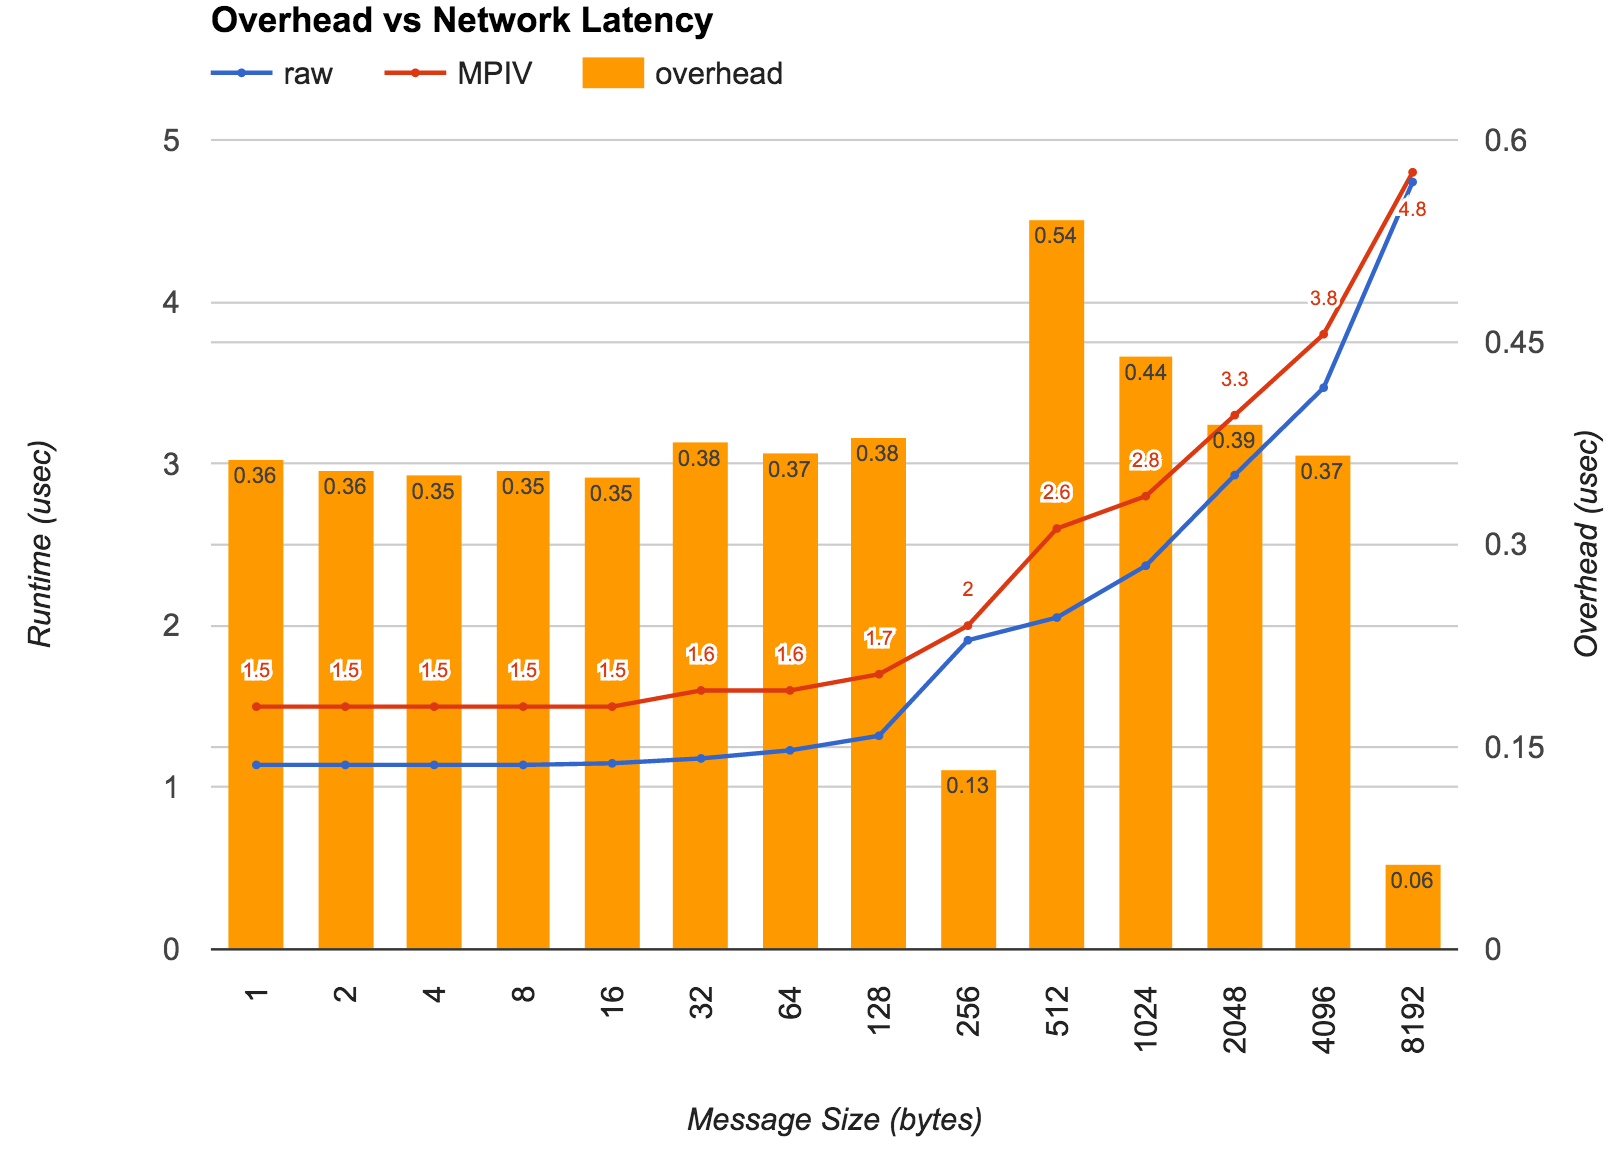
\includegraphics[width=0.4\textwidth]{fig/overhead.png}
  \caption{Overhead in comparison to raw network latency.}
\end{figure}

\subsection{Micro-benchmarks}
In this section, we measure overall latency and message rate of the runtime
under single and multi-threaded executions. We use the OSU benchmarks for
latency measurement and Sandia multi-threaded benchmarks for messsage rate
measurement. We compare our runtime (denoted as MPIV) with MVAPICH2.

%\begin{figure}
%  \centering 
%  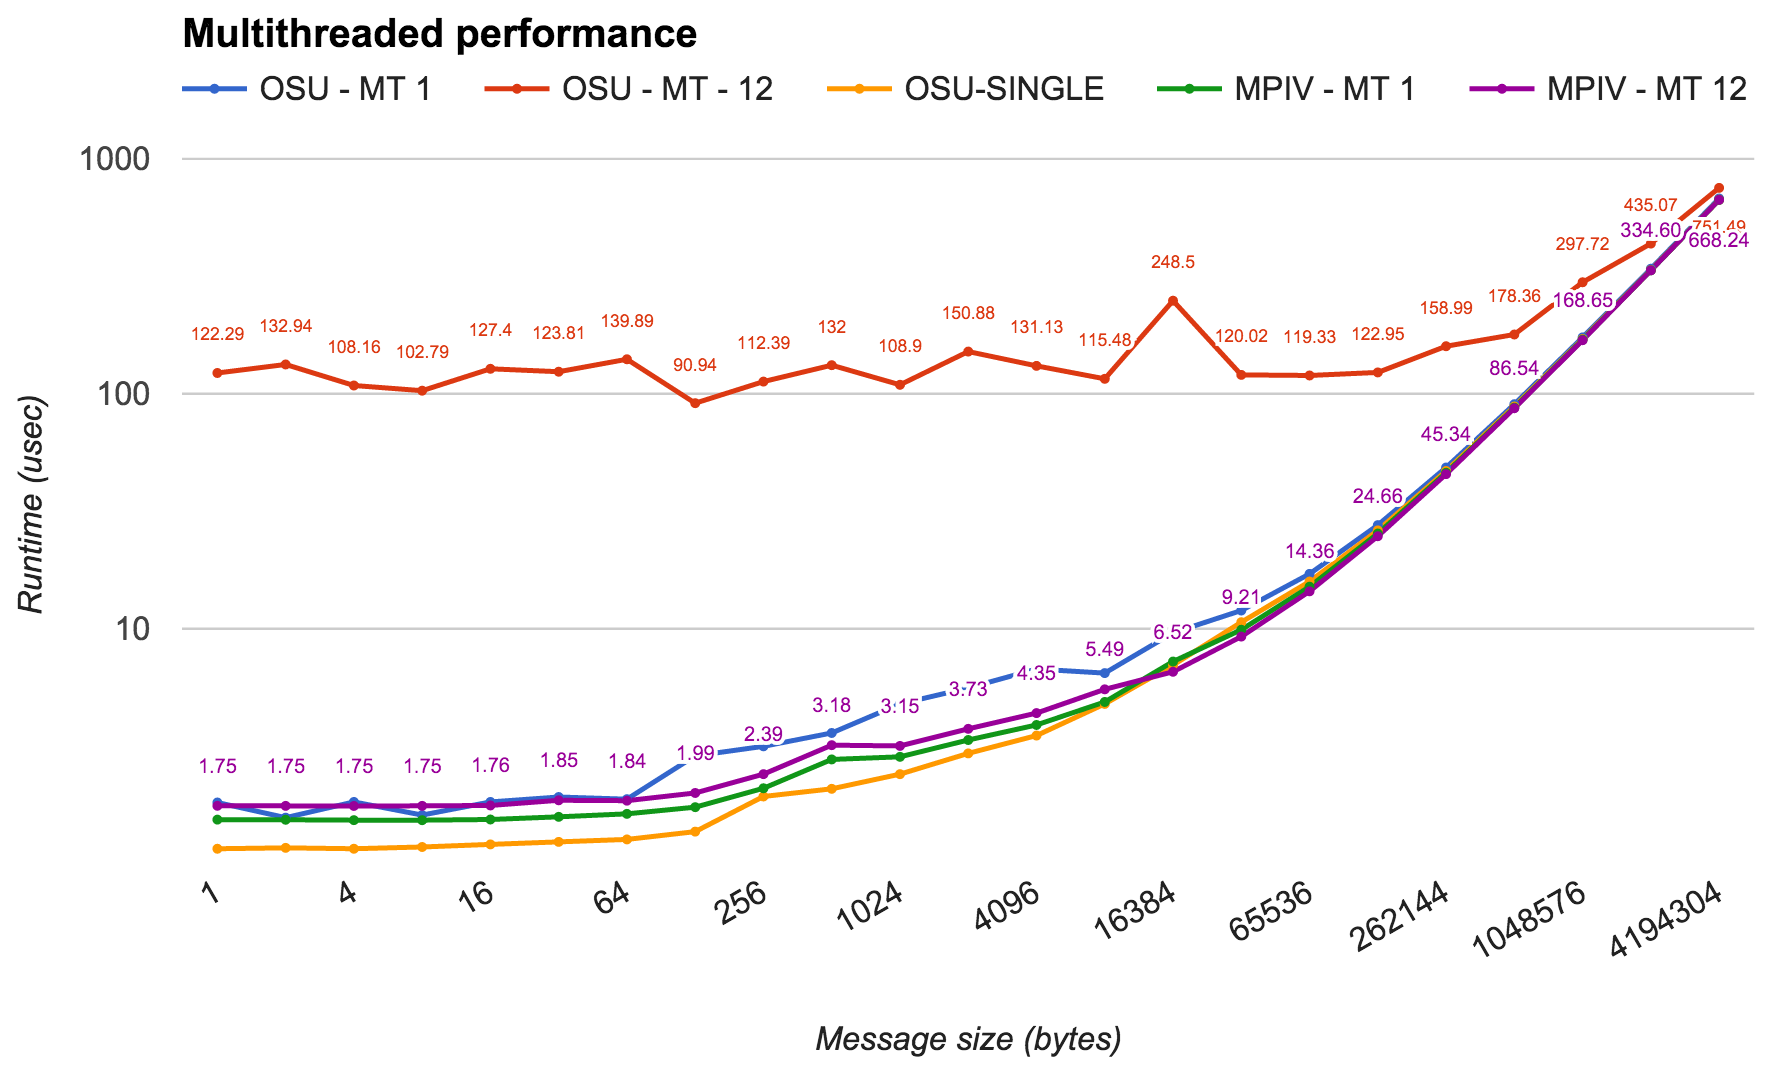
\includegraphics[width=0.5\textwidth]{fig/pingpong.png}
%  \caption{Comparing latency using OSU benchmarks using 1-thread
%  in 1-worker and 12-threads in 12-workers.} 
%\end{figure}

\subsection{Applications}
We shows BFS, UTS, Stencil.

